\documentclass[10pt]{beamer}

\usetheme{metropolis}
\usepackage{appendixnumberbeamer}

\usepackage{booktabs}
\usepackage[scale=2]{ccicons}

\usepackage{pgfplots}
\usepgfplotslibrary{dateplot}

\usepackage{xspace}
\newcommand{\themename}{\textbf{\textsc{metropolis}}\xspace}

\title{A brief overview of mathematical optimization}
\subtitle{}
\date{\today}
\author{Paul Bouman}
\institute{Winter Workshop on Complex Systems 2022, Arc-et-Senans, France}

\metroset{block=fill}

\usepackage{minted}

\begin{document}

\maketitle

\begin{frame}{Table of contents}
  \setbeamertemplate{section in toc}[sections numbered]
  \tableofcontents[hideallsubsections]
\end{frame}

\section{Introduction}

\begin{frame}[fragile]{Examples}

What do these pictures have in common?

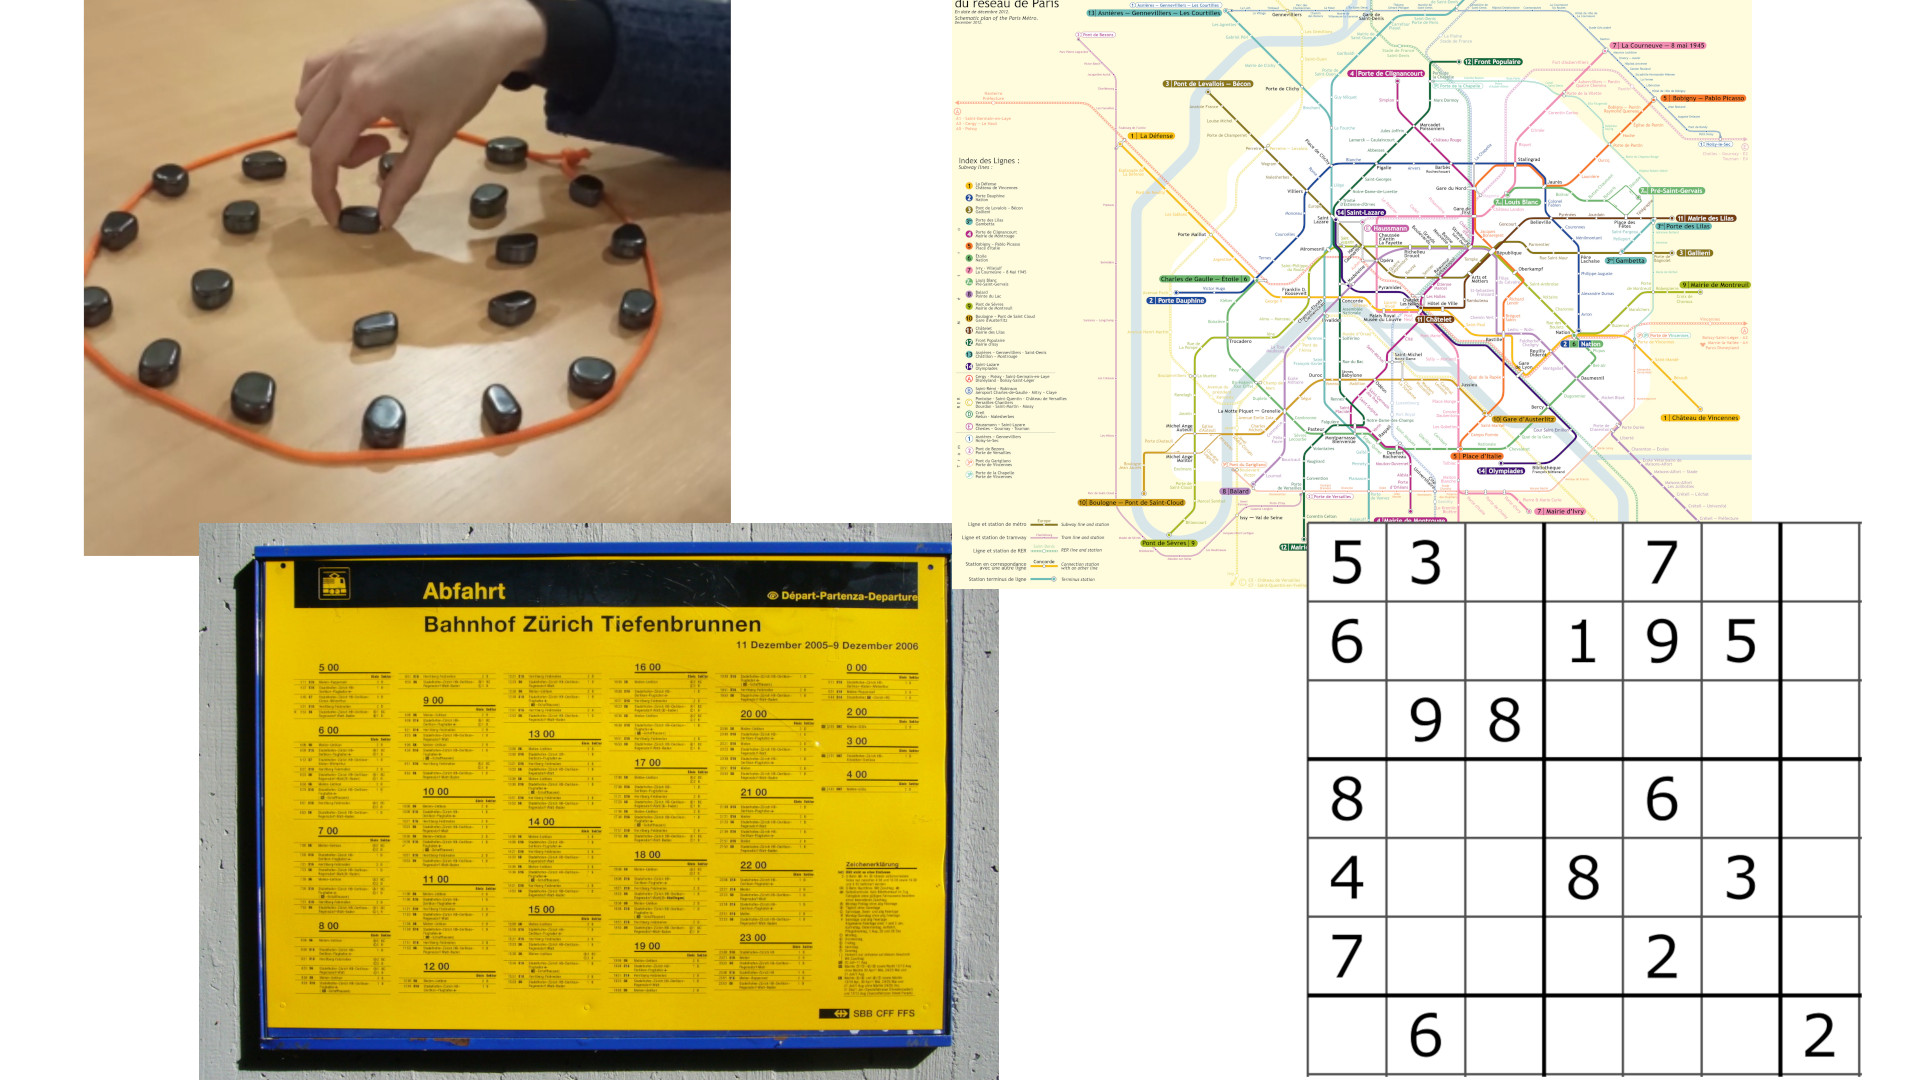
\includegraphics[width=0.8\textwidth]{examples.jpg}

{ \small \textbf{Attribution} \\
  \href{https://commons.wikimedia.org/wiki/File:Carte_M%C3%A9tro_de_Paris.jpg}{\underline{\color{cyan}Metro picture taken from Wikipedia}} \\
  \href{https://commons.wikimedia.org/wiki/File:FahrplanTiefenbrunnen.JPG}{\underline{\color{cyan}Timetable picture taken from Wikipedia}}
}

\end{frame}

\begin{frame}[fragile]{Examples}

Three important ingredients:

\begin{itemize}
	\item Coordinated/Centralized but \textbf{variable} decisions are needed
	\item Local or global rules \textbf{constrain} what combinations of decision are possible
	\item Optionally: \textbf{objective} it to make some measure of quality as \emph{good as possible}
\end{itemize}

\end{frame}

\begin{frame}[fragile]{Optimization}
	
\begin{block}{Optimization}
  \begin{enumerate}[<+- | alert@+>]
    \item Try to find a \textbf{feasible solution} that is \textbf{as good as possible}
    \item Provide reasoning why \textbf{no better solution can exist}
  \end{enumerate}
\end{block}

  \onslide<3-4>{Pendantic people could say that there is \emph{search} and that there is \emph{optimization}}

  \onslide<4>{The distance between the best solution found and the proof of the best possible is called an \textbf{optimization gap}}	
\end{frame}

\begin{frame}[fragile]{Optimization}

  Many concepts and approaches exists 

%  \begin{columns}[T,onlytextwidth]
%    \column{0.33\textwidth}
      \begin{block}{Concepts}
	  \begin{itemize}
		\item Logic Programming: variables are true/false, try to satisfy a formula
		\item Heuristics / Genetic Programming: start somewhere, iterate between small changes and accepting improvements
		\item Constraint Satisfaction: guess, then propagate over constraints to reduce variable domains, backtrack when stuck
		\item \textbf{Mathematical Programming}: 
	  \end{itemize}
	  \end{block}
%    \column{0.33\textwidth}
      \begin{block}{Flexibility}
		\begin{itemize}
			\item Non-linear programming: all kinds of equations, local or global optimum?
			\item Convex Programming: allow equations such that local and global optimum coincide
			\item \textbf{Linear Programming}: only allow linear equations
		\end{itemize}
	  \end{block}
%  \end{columns}

\end{frame}

\begin{frame}[fragile]{Linear Programming}

In my opinion \emph{Linear Programming} is a bit of a \emph{sweet spot}:

\begin{itemize}
	\item good to decent interpretability of decision models 
	\item surprisingly versatile decision modelling power
	\item decent opportunities for analytical and theoretical results 
	\item high quality (commercial) software available
\end{itemize}

\end{frame}

\section{Models and Examples}

\begin{frame}[fragile]{Basics}
\begin{block}{(Integer) Linear Programming}
\begin{itemize} 
	\item \textbf{Decision variables} with optional lower bound and upper bound, either \textbf{continuous} or \textbf{integer}. Variables that can be either $0$ or $1$ can model yes/no decisions and are called \textbf{binary} variables (special case of integer variables).
	\item \textbf{Objective function} to be minimize or maximized that is linear in terms of the variables
	\item \textbf{Constraints} that must be satisfied expressed using $\leq$, $=$ or $\geq$ where left and right hand side are linear in terms of the variables (or constant).
\end{itemize}
\end{block}
\end{frame}

\begin{frame}[fragile]{Basics}

With decision variables $x, y$ and $z$.

\begin{block}{Allowed}
\[\begin{array}{l}
\mbox{Minimize}~4 x - 2 y \\
3.14 x + 18 y \geq 4 \\
6 ( 4 x + 6 y ) \leq 2 z \\
4 x = 6 y
\end{array}\]
\end{block}

\begin{block}{Not allowed}
\[\begin{array}{l}
y ( 2 x - 3 z) \geq 2 \\
y + 2 x \neq z
\end{array}\]
\end{block}

However, there are many rewriting tricks. For example absolute values or the product of binary variables can often be dealt with.

\end{frame}

\begin{frame}[fragile]{Example: Maximum Independent Set}

  Given a network, what is the maximum number of nodes we can choose such that we do not select two neighbours?

  \begin{figure}
    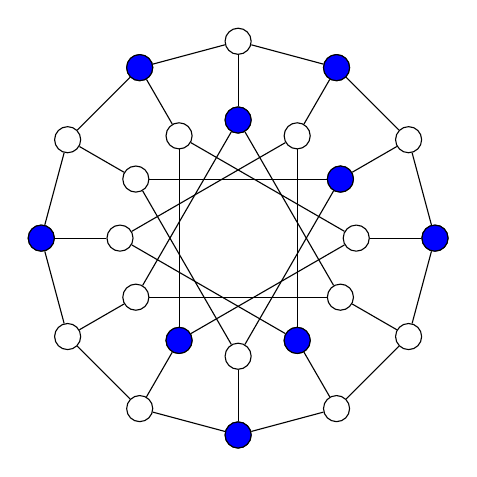
\begin{tikzpicture} 
		\node[draw,circle] (outer1) at ({360/12 * 1}:2.5cm) {};
		\node[draw,circle] (outer2) at ({360/12 * 2}:2.5cm) {};
		\node[draw,circle] (outer3) at ({360/12 * 3}:2.5cm) {};
		\node[draw,circle] (outer4) at ({360/12 * 4}:2.5cm) {};
		\node[draw,circle] (outer5) at ({360/12 * 5}:2.5cm) {};
		\node[draw,circle] (outer6) at ({360/12 * 6}:2.5cm) {};
		\node[draw,circle] (outer7) at ({360/12 * 7}:2.5cm) {};
		\node[draw,circle] (outer8) at ({360/12 * 8}:2.5cm) {};
		\node[draw,circle] (outer9) at ({360/12 * 9}:2.5cm) {};
		\node[draw,circle] (outer10) at ({360/12 * 10}:2.5cm) {};
		\node[draw,circle] (outer11) at ({360/12 * 11}:2.5cm) {};
		\node[draw,circle] (outer12) at (0:2.5cm) {};
		\node[draw,circle] (inner1) at ({360/12 * 1}:1.5cm) {};
		\node[draw,circle] (inner2) at ({360/12 * 2}:1.5cm) {};
		\node[draw,circle] (inner3) at ({360/12 * 3}:1.5cm) {};
		\node[draw,circle] (inner4) at ({360/12 * 4}:1.5cm) {};
		\node[draw,circle] (inner5) at ({360/12 * 5}:1.5cm) {};
		\node[draw,circle] (inner6) at ({360/12 * 6}:1.5cm) {};
		\node[draw,circle] (inner7) at ({360/12 * 7}:1.5cm) {};
		\node[draw,circle] (inner8) at ({360/12 * 8}:1.5cm) {};
		\node[draw,circle] (inner9) at ({360/12 * 9}:1.5cm) {};
		\node[draw,circle] (inner10) at ({360/12 * 10}:1.5cm) {};
		\node[draw,circle] (inner11) at ({360/12 * 11}:1.5cm) {};
		\node[draw,circle] (inner12) at (0:1.5cm) {};
		\draw[-] (outer1) to (inner1);
		\draw[-] (outer2) to (inner2);
		\draw[-] (outer3) to (inner3);
		\draw[-] (outer4) to (inner4);
		\draw[-] (outer5) to (inner5);
		\draw[-] (outer6) to (inner6);
		\draw[-] (outer7) to (inner7);
		\draw[-] (outer8) to (inner8);
		\draw[-] (outer9) to (inner9);
		\draw[-] (outer10) to (inner10);
		\draw[-] (outer11) to (inner11);
		\draw[-] (outer12) to (inner12);
		\draw[-] (outer1) to (outer2);
		\draw[-] (outer2) to (outer3);
		\draw[-] (outer3) to (outer4);
		\draw[-] (outer4) to (outer5);
		\draw[-] (outer5) to (outer6);
		\draw[-] (outer6) to (outer7);
		\draw[-] (outer7) to (outer8);
		\draw[-] (outer8) to (outer9);
		\draw[-] (outer9) to (outer10);
		\draw[-] (outer10) to (outer11);
		\draw[-] (outer11) to (outer12);
		\draw[-] (outer12) to (outer1);
		\draw[-] (inner1) to (inner5);
		\draw[-] (inner2) to (inner6);
		\draw[-] (inner3) to (inner7);
		\draw[-] (inner4) to (inner8);
		\draw[-] (inner5) to (inner9);
		\draw[-] (inner6) to (inner10);
		\draw[-] (inner7) to (inner11);
		\draw[-] (inner8) to (inner12);
		\draw[-] (inner9) to (inner1);
		\draw[-] (inner10) to (inner2);
		\draw[-] (inner11) to (inner3);
		\draw[-] (inner12) to (inner4);
		\onslide<2-3> {
			\node[draw,circle,fill=blue] at ({360/12 * 2}:2.5cm) {};
			\node[draw,circle,fill=blue] at ({360/12 * 4}:2.5cm) {};
			\node[draw,circle,fill=blue] at ({360/12 * 6}:2.5cm) {};
			\node[draw,circle,fill=blue] at ({360/12 * 9}:2.5cm) {};
			\node[draw,circle,fill=blue] at (0:2.5cm) {};		
			\node[draw,circle,fill=blue] at ({360/12 * 1}:1.5cm) {};
			\node[draw,circle,fill=blue] at ({360/12 * 3}:1.5cm) {};
			\node[draw,circle,fill=blue] at ({360/12 * 8}:1.5cm) {};
			\node[draw,circle,fill=blue] at ({360/12 * 10}:1.5cm) {};
	}
		\end{tikzpicture}
	\end{figure}

	\onslide<3>{
	{\small Possible application: where to plant trees that require distance
	
	(nodes are locations, edges indicate conflicts)}
	}
\end{frame}

\begin{frame}[fragile]{Example: Maximum Independent Set}
\begin{block}{Notation}
	A graph $G = (V,E)$ where $V$ contains nodes and $E$ contains edges.
\end{block}

\textbf{Variables: }For each node $v$ in $V$, introduce a binary variable $x_v$ and let us say that
\[
	x_v = \left\{ \begin{array}{ll} 1 & \mbox{ if } $v$ \mbox{ is selected } \\ 0 & \mbox{ otherwise } \end{array} \right.
\]

\textbf{Objective: }
\[
	\mbox{Maximize }~\sum_{v \in V} x_v
\]

\textbf{Constraints: } for each edge $(v,w) \in E$:
\[
	x_v + x_w \leq 1
\]

\end{frame}


\begin{frame}[fragile]{Exercise: Minimum Dominating Set}
	Choose the minimum number of nodes such that each node is either selected or has a selected neighbour

	\begin{figure}
		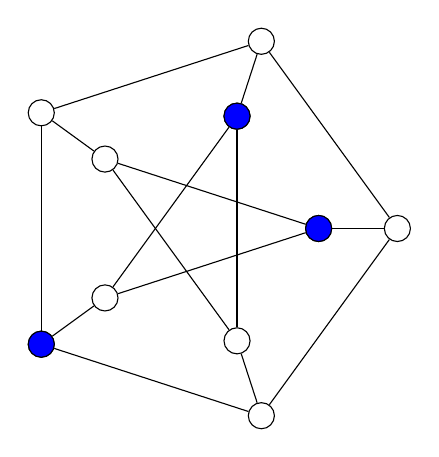
\begin{tikzpicture}
			\node[draw,circle] (outer1) at (0:2.5cm) {};
			\node[draw,circle] (outer2) at ({360/5 * 1}:2.5cm) {};
			\node[draw,circle] (outer3) at ({360/5 * 2}:2.5cm) {};
			\node[draw,circle] (outer4) at ({360/5 * 3}:2.5cm) {};
			\node[draw,circle] (outer5) at ({360/5 * 4}:2.5cm) {};
			\node[draw,circle] (inner1) at (0:1.5cm) {};
			\node[draw,circle] (inner2) at ({360/5 * 1}:1.5cm) {};
			\node[draw,circle] (inner3) at ({360/5 * 2}:1.5cm) {};
			\node[draw,circle] (inner4) at ({360/5 * 3}:1.5cm) {};
			\node[draw,circle] (inner5) at ({360/5 * 4}:1.5cm) {};
			\draw[-] (outer1) to (outer2);
			\draw[-] (outer2) to (outer3);
			\draw[-] (outer3) to (outer4);
			\draw[-] (outer4) to (outer5);
			\draw[-] (outer5) to (outer1);
			\draw[-] (inner1) to (inner3);
			\draw[-] (inner2) to (inner4);
			\draw[-] (inner3) to (inner5);
			\draw[-] (inner4) to (inner1);
			\draw[-] (inner5) to (inner2);
			\draw[-] (outer1) to (inner1);
			\draw[-] (outer2) to (inner2);
			\draw[-] (outer3) to (inner3);
			\draw[-] (outer4) to (inner4);
			\draw[-] (outer5) to (inner5);
			\onslide<2-3> {
				\node[draw,circle,fill=blue] (inner1) at (0:1.5cm) {};
				\node[draw,circle,fill=blue] (inner2) at ({360/5 * 1}:1.5cm) {};
				\node[draw,circle,fill=blue] (outer4) at ({360/5 * 3}:2.5cm) {};			
			}
		\end{tikzpicture}
	\end{figure}

	\onslide<3>{
	\small Possible application: where to locate ambulance depots
	
	(how would you model this?)
	}
\end{frame}

\begin{frame}[fragile]{Example: Minimum Cut}
	Remove minimum number of edges such that two given nodes are disconnected
	\begin{figure}
		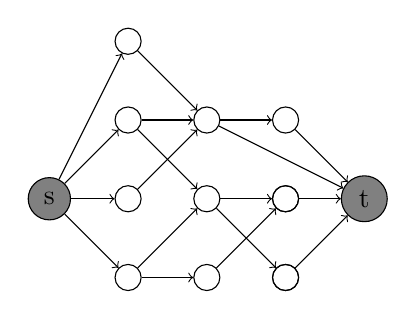
\begin{tikzpicture}
			\node[draw,circle,fill=gray] (s) at (0,1) {s};
			\node[draw,circle] (v1) at (1,0) {};
			\node[draw,circle] (v2) at (1,1) {};
			\node[draw,circle] (v3) at (1,2) {};
			\node[draw,circle] (v4) at (1,3) {};
			\node[draw,circle] (w1) at (2,0) {};
			\node[draw,circle] (w2) at (2,1) {};
			\node[draw,circle] (w3) at (2,2) {};
			\node[draw,circle] (u1) at (3,0) {};
			\node[draw,circle] (u2) at (3,1) {};
			\node[draw,circle] (u3) at (3,2) {};
			\node[draw,circle] (u1) at (3,0) {};
			\node[draw,circle] (u2) at (3,1) {};
			\node[draw,circle,fill=gray] (t) at (4,1) {t};
			\draw[->] (s) to (v1);
			\draw[->] (s) to (v2);
			\draw[->] (s) to (v3);
			\draw[->] (s) to (v4);
			\draw[->] (v1) to (w1);
			\draw[->] (v1) to (w2);
			\draw[->] (v2) to (w3);
			\draw[->] (v3) to (w2);
			\draw[->] (v3) to (w3);
			\draw[->] (v4) to (w3);
			\draw[->] (w1) to (u2);
			\draw[->] (w2) to (u1);
			\draw[->] (w2) to (u2);
			\draw[->] (w3) to (t);			
			\draw[->] (w3) to (u3);			
			\draw[->] (u1) to (t);
			\draw[->] (u2) to (t);
			\draw[->] (u3) to (t);			
		\end{tikzpicture}
	\end{figure}
\end{frame}


\begin{frame}[fragile]{Example: Minimum Cut}

\begin{block}{Notation}
	A directed graph $G = (V,A)$ where $V$ contains nodes and $A$ contains arcs.
\end{block}

\textbf{Variables: } for each arc $(v,w) \in A$ a variable $x_{vw}$ and for each node $u \in V$ a variable $z_u$:
\[
	x_{vw} = \left\{ \begin{array}{ll} 1 & \mbox{ if } (v,w) \mbox{ is cut } \\ 0 & \mbox{ otherwise } \end{array} \right. ~ , ~
	z_u = \left\{ \begin{array}{ll} 1 & \mbox{ if } v \mbox{ is connected to } s \\ 0 & \mbox{ otherwise } \end{array} \right.
\] 

\textbf{Objective: }
\[
	\mbox{ Minimize } ~ \sum_{(v,w) \in A} x_{vw}
\]

\textbf{Constraints: } for each arc $(v,w) \in A$ for propagation of connectivity
\[
  z_w \geq z_v - x_{vw}
\]
and also fix the connectivity state of $s$ and $t$:
\[
x_s = 1 ~ , ~ x_t = 0
\]

\end{frame}

\section{How is it solved}

\begin{frame}[fragile]{How to solve it}
\begin{figure}

	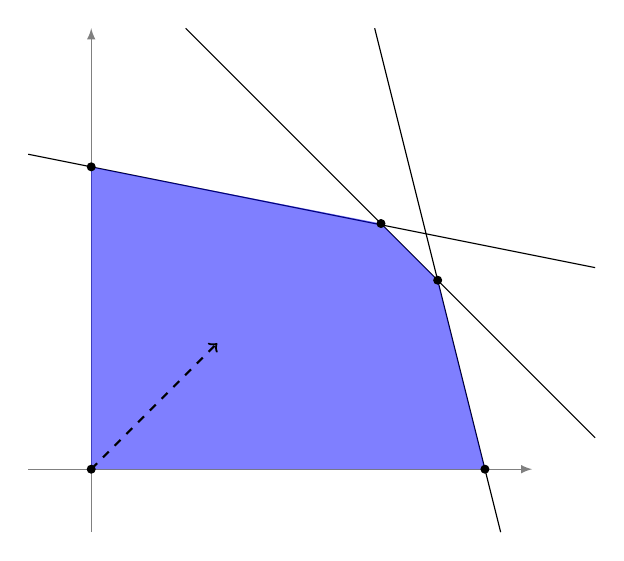
\begin{tikzpicture}[scale=0.8]
		\coordinate (Origin)   at (0,0);
		\coordinate (XAxisMin) at (-1,0);
		\coordinate (XAxisMax) at (7,0);
		\coordinate (YAxisMin) at (0,-1);
		\coordinate (YAxisMax) at (0,7);
		\draw [thin, gray,-latex] (XAxisMin) -- (XAxisMax);% Draw x axis
		\draw [thin, gray,-latex] (YAxisMin) -- (YAxisMax);% Draw y axis

		
		\onslide<2-7>{\draw [-] (-1,5) -- (8, 3.2);} % constraint 1
		\onslide<3-7>{\draw [-] (1.5,7) -- (8, 0.5);} % constraint 2
		\onslide<4-7>{\draw [-] (4.5,7) -- (6.5, -1);} % constraint 2

		\onslide<5-7>{\fill [opacity=0.5,blue] (0,0) -- (0,4.8) -- (4.6,3.9) -- (5.5,3) -- (6.25,0) -- (0,0);}

		\onslide<7>{
		\node[draw,circle,inner sep=1pt,fill] at (4.6,3.9){};
		\node[draw,circle,inner sep=1pt,fill] at (5.5,3){};
		\node[draw,circle,inner sep=1pt,fill] at (0,4.8){};
		\node[draw,circle,inner sep=1pt,fill] at (6.25,0){};
		\node[draw,circle,inner sep=1pt,fill] at (0,0){};
		}

		\onslide<6-7>{\draw [->,dashed,thick] (0,0) -- (2,2);}

%		\onslide<3>{
%			\foreach \x in {0,1,...,7}{% Two indices running over each
%				\foreach \y in {0,1,...,7}{% node on the grid we have drawn 
%					\node[draw,circle,inner sep=0.5pt,fill] at (\x,\y) {};
%				}
%			}
%		}
	\end{tikzpicture}
\end{figure}

\end{frame}

\begin{frame}[fragile]{How to solve it}

The \textbf{Simplex Algorithm} walks from the intersection points on the boundary of the feasible region in the direction of the objective function.

There are four cases
\begin{itemize}
	\item The optimal solution is at a intersection point.
	\item The objective vector is orthogonal to a line segment (hyperplane): all the points on this line segment (hyperplane) are optimal.
	\item The feasible region is empty and you have no solution
	\item The feasible region is unbounded and the optimal solution is a \emph{ray} rather than a point.
\end{itemize}

\uncover<2>{But what about integer solutions?}
\end{frame}

\begin{frame}[fragile]{How to solve it - integer variables}
\begin{figure}
	
	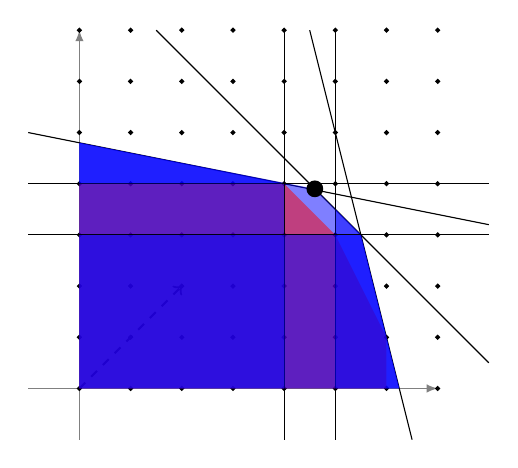
\begin{tikzpicture}[scale=0.65]
		\coordinate (Origin)   at (0,0);
		\coordinate (XAxisMin) at (-1,0);
		\coordinate (XAxisMax) at (7,0);
		\coordinate (YAxisMin) at (0,-1);
		\coordinate (YAxisMax) at (0,7);
		\draw [thin, gray,-latex] (XAxisMin) -- (XAxisMax);% Draw x axis
		\draw [thin, gray,-latex] (YAxisMin) -- (YAxisMax);% Draw y axis

		
		\draw [-] (-1,5) -- (8, 3.2); % constraint 1
		\draw [-] (1.5,7) -- (8, 0.5); % constraint 2
		\draw [-] (4.5,7) -- (6.5, -1); % constraint 2

		\draw [->,dashed,thick] (0,0) -- (2,2); % the objective

		\foreach \x in {0,1,...,7}{% Two indices running over each
			\foreach \y in {0,1,...,7}{% node on the grid we have drawn 
				\node[draw,circle,inner sep=0.5pt,fill] at (\x,\y) {};
			}
		}

		\onslide<1>{
			\fill [opacity=0.5,blue] (0,0) -- (0,4.8) -- (4.6,3.9) -- (5.5,3) -- (6.25,0) -- (0,0);
		}

		
		\onslide<2>{
			\fill [opacity=0.5,red] (0,0) -- (0,4) -- (4,4) -- (5,3) -- (6,1) -- (6,0) -- (0,0);
		
		}

		\onslide<1-2>{
					\node[draw,circle,inner sep=2pt,fill] at (4.6,3.9){};
		}
		
		\onslide<3>{
			\draw [-] (4,7) -- (4, -1); % constraint 2
			\draw [-] (5,7) -- (5, -1); % constraint 2
			\fill [opacity=0.5,blue] (0,0) -- (0,4.8) -- (4,4) -- (4,0) -- (0,0) ;
			\fill [opacity=0.5,blue] (5,0) -- (5,3.5) -- (5.5,3) -- (6.25,0) -- (5,0) ;
		}
		
		\onslide<4>{
			\draw [-] (-1,3) -- (8, 3); % constraint 2
			\draw [-] (-1,4) -- (8, 4); % constraint 2
			\fill [opacity=0.5,blue] (0,0) -- (0,3) -- (5.5,3) -- (6.25,0) -- (0,0) ;
			\fill [opacity=0.5,blue] (0,4) -- (0,4.8) -- (4,4) -- (0,4) ;
		}


	\end{tikzpicture}
\end{figure}

	{\small
	\only<1>{Simplex algorithm may give use fractional solutions, even if we want (some) variables to be integer.
	\vspace{1.5em}
	}
	
	\only<2>{We do not know a good way to convert the fractional feasible space to an integer feasible space.
	\vspace{1.5em}}
	
	\only<3-4>{We can start with a fractional solution, and then split up the feasible spaces into two subspaces, and take the best solution in the two smaller spaces.
	            In this example we can either split on the $x$ or the $y$ variable}
	}

\end{frame}

\begin{frame}[fragile]{How to solve it - integer variables}

Try to solve the non-integer version as explained before, and split the problem in two if your solution is fractional.

For every variable you have to split the number of subproblems doubles, so this could lead to an exponential amount of work in the number of variables.

However, you can eliminate subproblems where the optimal fractional solution is worse than the best solution \emph{so far}, and only focus on sub-problems
where there is actually a potential gap to close. This is called \textbf{branch-and-bound}.

The decision on which variable to split can have a huge impact on the amount of work that is needed. Commercial solvers have invested insane amounts of effort in
developing tricks to do this in a clever way (among many other things).

\end{frame}

\section{Software}

\begin{frame}[fragile]{Solvers}

There are many linear programming and integer linear programming solvers,
but the quality varies wildly.

To create a good solver, there are many things to deal with:

\begin{itemize}
	\item Exploit that many constraint matrices are very sparse (i.e. many constraints deal with a small number of variables)
	\item Numerical precision
	\item Strategies for branching/splitting to obtain integer solutions
	\item Strategies to obtain intermediate integer solutions that allow you to eliminate irrelevant parts of the search space
	\item Preprocessing of the model to make it more compact/easier to solve
\end{itemize}

\end{frame}

\begin{frame}[fragile]{Solvers}
Since better optimization software can save large enterprises a lot of money, developers of commercial solvers invested a lot
of effort to learn all kinds of mathematical and emperical tricks to make better solvers to tackle larger problems.
Open source efforts were typically developed by volunteers working in Academia.

For integer programming, the 2015 version of Guribo is in benchmarks 800000 ($8\cdot10^5$) times faster\footnote{according to \href{https://www.lnmb.nl/conferences/2015/programlnmbconference/LNMB-NGB_Bixby.pdf}{\color{cyan}\underline{a presentation}} by one of it's creators} than the 1991 version of
CPLEX, \textbf{on the same computer hardware}. 

This means that a problem that solves in an hour with a state-of-the-art solver, could take more than 90 years to solve on a simple one.

There are cases where researchers incorrectly conclude linear programming is \emph{intractable} based only on experiments with a simple solver.
\end{frame}

\begin{frame}[fragile]{Solvers}

Of course, it is good to be aware there is tension between \emph{open science} and \emph{closed source commercial packages} and \emph{black box methods}.
Whether this is a problem or not depends on what you try to achieve. Some points to consider

\begin{itemize}
	\item The mathematical model that is solved is known (you define it) and it can be validated that a solution is actually correct according to the model independently.
	\item Generally, the overarching approach of these solvers is known, but the clever tricks they use to find solutions faster is not
	\item Good solvers provide a lot of ways to track and influence what they are doing while they are solving, which provides some level of transparency.
\end{itemize} 

However, if you want to make your computational process easily reproducible for anyone, even companies and curious people not affiliated with a research institute,
an open source solver may be a better choice.

\end{frame}

\begin{frame}[fragile]{Solvers}

An overview of some interesting solvers for Linear Programming:

\begin{table}
\begin{tabular}{llllll}
\toprule
Solver & Models & Speed & Open Source & Academic & Commercial \\
\midrule
\href{https://projects.coin-or.org/Clp}{\color{cyan}\underline{COIN-OR Clp}} & LP & good & Yes & Free & Free \\
\href{https://github.com/coin-or/Cbc}{\color{cyan}\underline{COIN-OR Cbc}} & ILP & ok & Yes & Free & Free \\
\href{https://www.scipopt.org/}{\color{cyan}\underline{SCIP}} & ILP+ & good & Yes & Free & Paid \\
\href{https://www.ibm.com/analytics/cplex-optimizer}{\color{cyan}\underline{CPLEX}} & ILP+ & great & No & Free & Paid \\
\href{https://www.gurobi.com/}{\color{cyan}\underline{Gurobi}} & ILP+ & great & No & Free & Paid \\
\bottomrule
\end{tabular}
\end{table}

LP: linear programming, ILP: integer linear programming, \\ ILP+: also support for some non-linear models.

{CPLEX used to be state of the art, now Gurobi has the most active development.
An academic license for Gurobi requires authentication from a campus network, for CPLEX you can just install and use it after
creating an academic account.}

\end{frame}

\begin{frame}[fragile]{Using a Solver}

A good approach can be to use a package that is \emph{solver-agnostic}. That means you build your optimization model with the package, and
then can select which solver can be used. This way, you can easily switch between a free and a commercial solver (assuming both are available on your computer).

In Python, two popular options are \href{https://www.pyomo.org/}{\color{cyan}\underline{Pyomo}} and \href{https://github.com/coin-or/pulp}{\color{cyan}\underline{PuLP}}.
Pyomo is more abstract in modelling and providers abstract tools to transform your data into a model. PuLP is more low level and only allows you to define variables, constraints
and the objective in a straightforward manner. For Julia, \href{https://jump.dev}{\color{cyan}\underline{JuMP}} is a popular option.

The downside of using a solver-agnostic package is that you lose some access to the internals of a particular solver, but that is typically only a concern if you want
to implement very advanced techniques.

\end{frame}

\begin{frame}[fragile]{Pyomo code example}

\begin{minted}[fontsize=\scriptsize]{python}
from pyomo.environ import *

model = ConcreteModel()

# declare decision variables
x = Var(domain=Reals,bounds=(0,4))
y = Var(domain=Reals,bounds=(-1,1))
z = Var(domain=NonNegativeReals)

# declare objective
model.profit = Objective(expr = x + 4*y + 9*z, sense = minimize)

# declare constraints
model.c1 = Constraint(expr = x + y <= 5)
model.c2 = Constraint(expr = x + z >= 10)
model.c3 = Constraint(expr = -y + z == 7)

# solve
SolverFactory('cplex').solve(model)
print("objective=", model.profit())
\end{minted}
\end{frame}

\begin{frame}[fragile]{PuLP code example}
\begin{minted}[fontsize=\scriptsize]{python}
from pulp import *

prob = LpProblem("test1", LpMinimize)

# Variables
x = LpVariable("x", 0, 4) # 0 <= x <= 4
y = LpVariable("y", -1, 1) # -1 <= y <= 1
z = LpVariable("z", 0) # 0 <= z

# Objective (the name at the end is facultative)
prob += x + 4 * y + 9 * z, "obj"

# Constraints (the names at the end are facultative)
prob += x + y <= 5, "c1"
prob += x + z >= 10, "c2"
prob += -y + z == 7, "c3"

# Solve the problem using the default solver
prob.solve()  # use prob.solve(CPLEX()) instead to use CPLEX 

# Print the value of the objective
print("objective=", value(prob.objective))
\end{minted}

{\scriptsize (Based on {\color{cyan}\underline{\url{https://github.com/coin-or/pulp/blob/master/examples/test1.py}}})}

\end{frame}

\begin{frame}[fragile]{Implementing Models}

To construct models based on graphs, you typically want to create a list or a dictionary to hold variables and fill these
based on data about nodes/edges.

For more examples and explanation, it makes sense to read the documentation:
\begin{itemize}
	\item \href{https://pyomo.readthedocs.io}{\color{cyan}\underline{Pyomo documentation}}
	\item \href{https://jckantor.github.io/ND-Pyomo-Cookbook/}{\color{cyan}\underline{Pyomo cookbook}}
	\item \href{https://coin-or.github.io/pulp/}{\color{cyan}\underline{PuLP documentation}}
\end{itemize}

\end{frame}

\section{Advanced Topics}

\begin{frame}[fragile]{Advanced topics}

Some advanced topics not discussed in this tutorial:

\begin{itemize}
	\item \emph{Duality}: \small for an optimal solution to a continuous linear programming model there is an associated and closely connected \emph{dual} solution, that provides interesting information about the sensitivity of your currect solution to changes in the constraints.
	\item \emph{Column generation/Branch-and-Prize}: \small approaches where we consider a very large number of variables (e.g. one variable for every subset of nodes of a graph), but add only relevant variables iteratively based on information from the dual problem. Typically you do not need to enumerate all variables this way, but only consider a small number of them.
	\item \emph{Constraint generation/Branch-and-Cut}: \small approaches where we consider a very large number of constraints (e.g. one constraint for every subset of nodes of a graph). When a solution is found, we try to find a violated constraint. If one is found, we add it. If no violated constraint can be found for the current solution, we know the solution is valid.
\end{itemize}

\end{frame}

\section{Conclusion}

\begin{frame}[fragile]{Conclusion}

This tutorial gave a quick overview of (integer) linear programming.

\begin{itemize}
	\item Provides an interesting mix between modelling versatility and high quality tools to tackle the models
	\item Simplicity of equations does provide opportunities to have some analytical results and helps with interpretability
	\item Commercial solvers are a lot faster, but free for academics (in particular if you have integer variables)
	\item Many packages that allow you to build models and swap which solver you use to solve them.
\end{itemize}

\begin{center}\large Thanks for your attention!\end{center}

\end{frame}

\section*{Solutions}

\begin{frame}[fragile]{Solution: Maximum Dominating Set}

\begin{block}{Notation}
	\begin{itemize}
		\item A graph $G = (V,E)$ where $V$ contains nodes and $E$ contains edges.
		\item For a node $v$, $\delta(v)$ gives us the neigbours
	\end{itemize}
\end{block}


\textbf{Variables: }For each node $v$ in $V$, introduce a binary variable $x_v$ and let us say that
\[
	x_v = \left\{ \begin{array}{ll} 1 & \mbox{ if } $v$ \mbox{ is selected } \\ 0 & \mbox{ otherwise } \end{array} \right.
\]

\textbf{Objective: }
\[
	\mbox{Minimize }~\sum_{v \in V} x_v
\]

\textbf{Constraints: } for each node $v \in V$:
\[
	x_v + \sum_{w \in \delta(v)} x_w \geq 1
\]

\end{frame}

%%%%%%%%% Stuff to delete later %%%%%%%%

\end{document}
